\subsection{Parte 2: circuito RLC in corrente alternata}

In accordo alla notazione utilizzata nella Parte 1, le funzioni di trasferimento sono parametrizzate e stimate utilizzando i parametri meccanici caratteristici di un sistema oscillante ad un grado di libertà: pulsazione propria e coefficiente di smorzamento. Le stime dei parametri elettrici di resistenza, induttanza e capacità sono ricavate operando una riparametrizzazione, e i relativi errori, ottenuti in accordo con l'approssimazione delle formule di propagazione.

In questa sezione le funzioni di trasferimento indicate con 
$f_{k}(w) = \frac{V_k}{V_A}$ si intendono quelle relative alla differenza di potenziale ai capi del generico componente $k$ sul segnale in ingresso $V_A$.


%%%%%%%%%%%%%%%%%%%%%%%%%%%%%%%%%%%%%%%%%%%%%%%%%%%%%%%%%%
%%%%%%%%%%%%%%%%%%%%%%% Resistenza



\subsubsection{Resistenza}

Funzione di trasferimento.
Si indica con $R$ la resistenza del resistore e con $r$ le altre resistenze (generatore, induttore).
$L$ l'induttanza e $C$ la capacità.

\begin{align*}
f_{R}(w) = \frac{V_{R}}{V_{A}} &= \frac{R}{(r+R) + j(wL - \frac{1}{wC})} 
= \frac{1}{(1+r/R) + \frac{j}{2\gamma}(w - \frac{w_0^2}{w})}
\end{align*}

Modulo e fase.
Posto $ y(w) = \frac{w - \frac{w_0^2}{w}}{2\gamma} $, e 
$ k = (1+r/R)$

\begin{align*}
& |\frac{V_{R}}{V_{A}}|  = ( y(w)^2 + k^2)^{-\frac{1}{2}}
& Arg\frac{V_{R}}{V_{A}} = \arctan( - \frac{y(w)}{k} )
\end{align*}

I parametri incogniti oggetto di stima sono
$ w_0^2 $, $\gamma$ e $r/R$, da cui si ricavano i parametri elettrici di interesse,

\begin{align*}
    & r = (\frac{ r }{R}) R
    & L =  \frac{r+R}{\gamma}\\
    & C = \frac{1}{L w_{0}^{2}}
\end{align*}

dove $R$, la resistenza del resistore, è oggetto di misura diretta, perciò non proveniente da stima. 

Di seguito i dati racolti e il loro grafico con la funzione adattata.


\begin{table}[H]
\begin{center}
\begin{tabular}{|r|r|r|r|r|l|r|r|r|r|r|}
\hline
\multicolumn{1}{|l|}{Freq} & \multicolumn{1}{l|}{Va} & \multicolumn{1}{l|}{Vb} & \multicolumn{1}{l|}{Fase } & \multicolumn{1}{l|}{Err Fase} &  & \multicolumn{1}{l|}{Freq} & \multicolumn{1}{l|}{Va} & \multicolumn{1}{l|}{Vb} & \multicolumn{1}{l|}{Fase } & \multicolumn{1}{l|}{Err Fase} \\ \hline
\multicolumn{1}{|l|}{Hz} & \multicolumn{1}{l|}{V} & \multicolumn{1}{l|}{V} & \multicolumn{1}{l|}{$\mu s$} & \multicolumn{1}{l|}{$\pm \mu s$} &  & \multicolumn{1}{l|}{Hz} & \multicolumn{1}{l|}{V} & \multicolumn{1}{l|}{V} & \multicolumn{1}{l|}{$\mu s$} & \multicolumn{1}{l|}{$\pm \mu s$} \\ \hline
\multicolumn{1}{|c|}{$\pm 1$} & \multicolumn{1}{c|}{$\pm 0.2$} & \multicolumn{1}{c|}{$\pm 0.08$} & \multicolumn{1}{l|}{} & \multicolumn{1}{l|}{} &  & \multicolumn{1}{c|}{$\pm 1$} & \multicolumn{1}{c|}{$\pm 0.2$} & \multicolumn{1}{c|}{$\pm 0.08$} & \multicolumn{1}{l|}{} & \multicolumn{1}{l|}{} \\ \hline
50 & 10.2 & 0.15 & 4900 & 200 &  & 3500 & 10.4 & 8.48 & -21 & 2 \\ \hline
100 & 10.2 & 0.30 & 2440 & 80 &  & 4000 & 10.6 & 7.44 & -28 & 4 \\ \hline
500 & 10.2 & 1.52 & 450 & 20 &  & 4500 & 10.6 & 6.48 & -30 & 2 \\ \hline
1000 & 10.4 & 3.20 & 192 & 8 &  & 5500 & 10.6 & 5.04 & -30 & 2 \\ \hline
1500 & 10.6 & 5.20 & 106 & 4 &  & 6500 & 10.8 & 4.16 & -28 & 2 \\ \hline
2000 & 10.6 & 7.44 & 52 & 4 &  & 7500 & 10.8 & 3.60 & -25 & 2 \\ \hline
2200 & 10.4 & 8.16 & 37 & 2 &  & 8500 & 10.8 & 3.12 & -24 & 2 \\ \hline
2500 & 10.2 & 9.04 & 19 & 2 &  & 9500 & 10.6 & 2.72 & -23 & 2 \\ \hline
2600 & 10.2 & 9.28 & 4 & 2 &  & 12000 & 10.6 & 2.16 & -18 & 2 \\ \hline
3000 & 10.5 & 9.28 & -6 & 2 &  & 20000 & 10.6 & 1.24 & -11.8 & 0.8 \\ \hline
3025 & 10.4 & 9.28 & -7 & 2 &  & 30000 & 10.6 & 0.84 & -8.4 & 0.4 \\ \hline
3050 & 10.4 & 9.28 & -9 & 2 &  & 40000 & 10.6 & 6.20 & -6.0 & 0.2 \\ \hline
3100 & 10.4 & 9.20 & -12 & 2 &  & 100000 & 10.5 & 0.20 & 2.48 & 0.08 \\ \hline

\end{tabular}
\end{center}
\caption{
Ddp e Fase ai capi del resistore.
Resistenza 1.000 (+50+50)  [$\Omega$].
Capacità  46    [$nF$].
Induttore 0.065 [$H$].
}
\label{tab:C2_P2_res}
\end{table}

\begin{figure}[H]
\centering
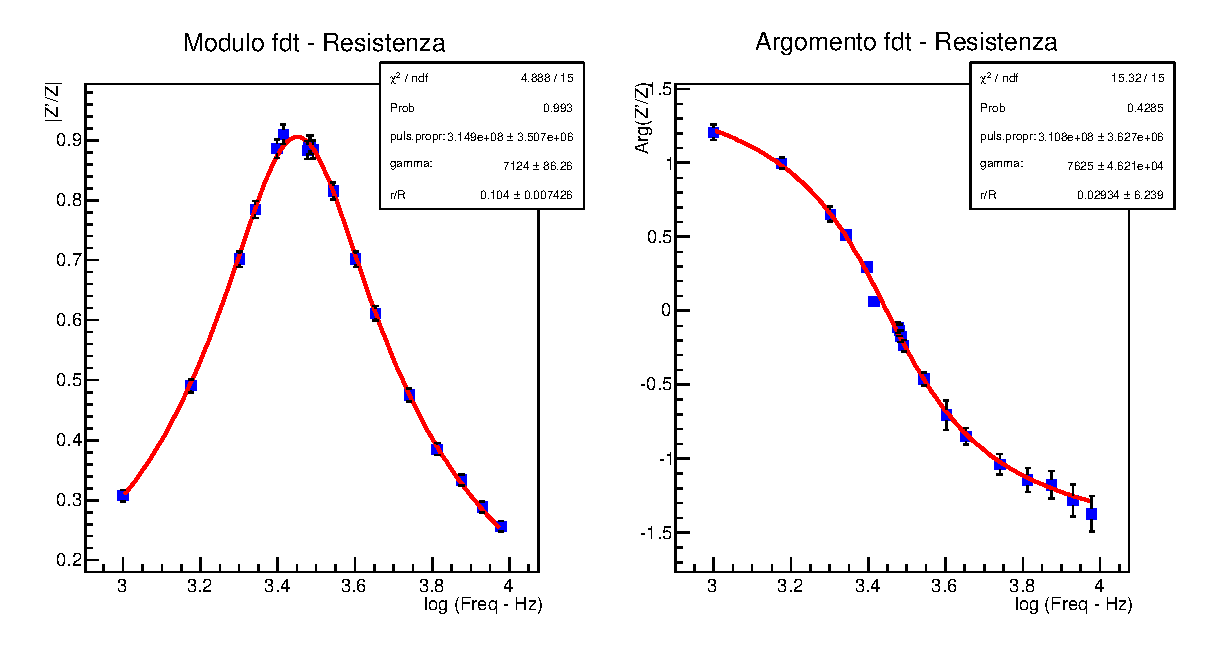
\includegraphics[scale=0.75]{Grafici/C4_P2_Res.eps}
\caption{
Circuito RLC serie.
AC.
Funzione di traferimento ai capi della resistenza.
}
\label{fig:C4_P2_Res}
\end{figure}







%%%%%%%%%%%%%%%%%%%%%%%%%%%%%%%%%%%%%%%%%%%%%%%%%%%%%%%%%%
%%%%%%%%%%%%%%%%%%%%%%% Capacità




\subsubsection{Capacità}

Funzione di trasferimento.
Si indica con $R$ la resistenza del resistore e con $r$ le altre resistenze (generatore, induttore).

\begin{align*}
f_{C}(w) = \frac{V_{C}}{V_{A}} 
= \frac{1}{ jwC ( (r+R) + j(wL - \frac{1}{wC}) ) }
= 
\frac{\frac{1}{w\frac{2\gamma}{w_0^2}}}
{( j(1+r/R) - \frac{1}{2\gamma}( w-\frac{w_0^2}{w} ) ) }.
\end{align*}

Modulo e fase.
Posto
$ y(w) = \frac{w - \frac{w_0^2}{w}}{2\gamma} $,
$ z(w) = \frac{1}{w\frac{2\gamma}{w_0^2}} $ e 
$ k = (1+r/R)$

\begin{align*}
& |\frac{V_{C}}{V_{A}}|  = z(w)( y(w)^2 + k^2)^{-\frac{1}{2}}
& Arg\frac{V_{C}}{V_{A}} = \arctan( \frac{k}{y(w)} )
\end{align*}


\begin{table}[H]
\begin{center}
\begin{tabular}{|r|r|r|r|r|}
\hline
\multicolumn{1}{|l|}{Freq} & \multicolumn{1}{l|}{Va} & \multicolumn{1}{l|}{Vb} & \multicolumn{1}{l|}{Fase } & \multicolumn{1}{l|}{Err Fase} \\ \hline
\multicolumn{1}{|l|}{Hz} & \multicolumn{1}{l|}{V} & \multicolumn{1}{l|}{V} & \multicolumn{1}{l|}{$\mu s$} & \multicolumn{1}{l|}{$\pm \mu s$} \\ \hline
\multicolumn{1}{|c|}{$\pm 1$} & \multicolumn{1}{c|}{$\pm 0.2$} & \multicolumn{1}{c|}{$\pm 0.08$} & \multicolumn{1}{l|}{} & \multicolumn{1}{l|}{} \\ \hline
20000 & 10.8 & 0.14 & 17.2 & 0.8 \\ \hline
10000 & 10.8 & 0.33 & 30.4 & 0.8 \\ \hline
8000 & 10.4 & 0.41 & 35.6 & 0.4 \\ \hline
6000 & 10.8 & 0.55 & 46 & 2 \\ \hline
4000 & 10.8 & 0.84 & 64 & 2 \\ \hline
2000 & 10.8 & 1.66 & 120 & 4 \\ \hline
1000 & 10.6 & 3.18 & 204 & 8 \\ \hline
500 & 10.4 & 5.48 & 330 & 20 \\ \hline
100 & 10.4 & 9.68 & 500 & 40 \\ \hline
50 & 10.4 & 10.00 & 440 & 40 \\ \hline
\end{tabular}
\end{center}
\caption{Ddp e Fase ai capi del condensatore.
Resistenza 11.000 (+50+50)  [$\Omega$].
Capacità  46    [$nF$].
Induttore 0.065 [$H$].}
\label{tab:C2_P2_cond}
\end{table}


\begin{figure}[H]
\centering
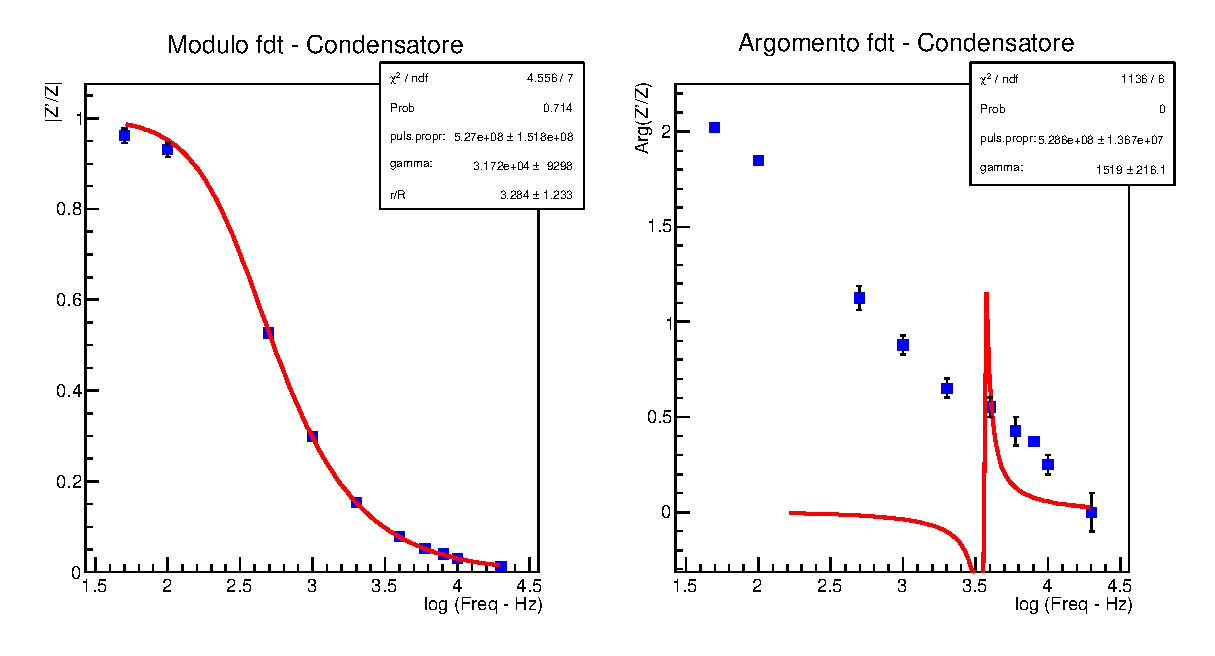
\includegraphics[scale=0.75]{Grafici/C4_P2_Cond.eps}
\caption{
Circuito RLC serie.
AC.
Funzione di traferimento ai capi della capacità.
}
\label{fig:C4_P2_Cond}
\end{figure}




%%%%%%%%%%%%%%%%%%%%%%%%%%%%%%%%%%%%%%%%%%%%%%%%%%%%%%%%%%
%%%%%%%%%%%%%%%%%%%%%%% Induttore




\subsubsection{Induttore}

Funzione di trasferimento.
Si indica con $R$ la resistenza del resistore e con $r$ le altre resistenze (generatore, induttore).

\begin{align*}
\frac{V_{L}}{V_{A}} 
= \frac{jwL}{ (r+R) + j(wL - \frac{1}{wC}) }
= 
\frac{\frac{w}{2\gamma}}
{ -j(1+r/R) + \frac{1}{2\gamma}( w-\frac{w_0^2}{w}) }.
\end{align*}

Modulo e fase.
Posto
$ y(w) = \frac{w - \frac{w_0^2}{w}}{2\gamma} $,
$ z(w) = \frac{w}{2\gamma} $ e 
$ k = (1+r/R)$

\begin{align*}
& |\frac{V_{C}}{V_{A}}|  = z(w)( y(w)^2 + k^2)^{-\frac{1}{2}}
& Arg\frac{V_{C}}{V_{A}} = \arctan( \frac{k}{y(w)} )
\end{align*}


\begin{table}[H]
\begin{center}
\begin{tabular}{|r|r|r|r|r|}
\hline
\multicolumn{1}{|l|}{Freq} & \multicolumn{1}{l|}{Va} & \multicolumn{1}{l|}{Vb} & \multicolumn{1}{l|}{Fase } & \multicolumn{1}{l|}{Err Fase} \\ \hline
\multicolumn{1}{|l|}{Hz} & \multicolumn{1}{l|}{V} & \multicolumn{1}{l|}{V} & \multicolumn{1}{l|}{$\mu s$} & \multicolumn{1}{l|}{$\pm \mu s$} \\ \hline
\multicolumn{1}{|c|}{$\pm 1$} & \multicolumn{1}{c|}{$\pm 0.2$} & \multicolumn{1}{c|}{$\pm 0.08$} & \multicolumn{1}{l|}{} & \multicolumn{1}{l|}{} \\ \hline
500 & 10.2 & 0.33 & 870 & 20 \\ \hline
1000 & 10.2 & 1.36 & 424 & 4 \\ \hline
2000 & 10.4 & 6.60 & 176 & 4 \\ \hline
20000 & 10.6 & 10.50 & 1 & 0.2 \\ \hline
30000 & 10.6 & 10.50 & 0.3 & 0.2 \\ \hline
\end{tabular}
\end{center}
\caption{Ddp e Fase ai capi dell'induttore.
Resistenza 1.000 (+50+50)  [$\Omega$].
Capacità  46    [$nF$].
Induttore 0.065 [$H$].
}
\label{tab:C2_P2_ind}
\end{table}

\begin{figure}[H]
\centering
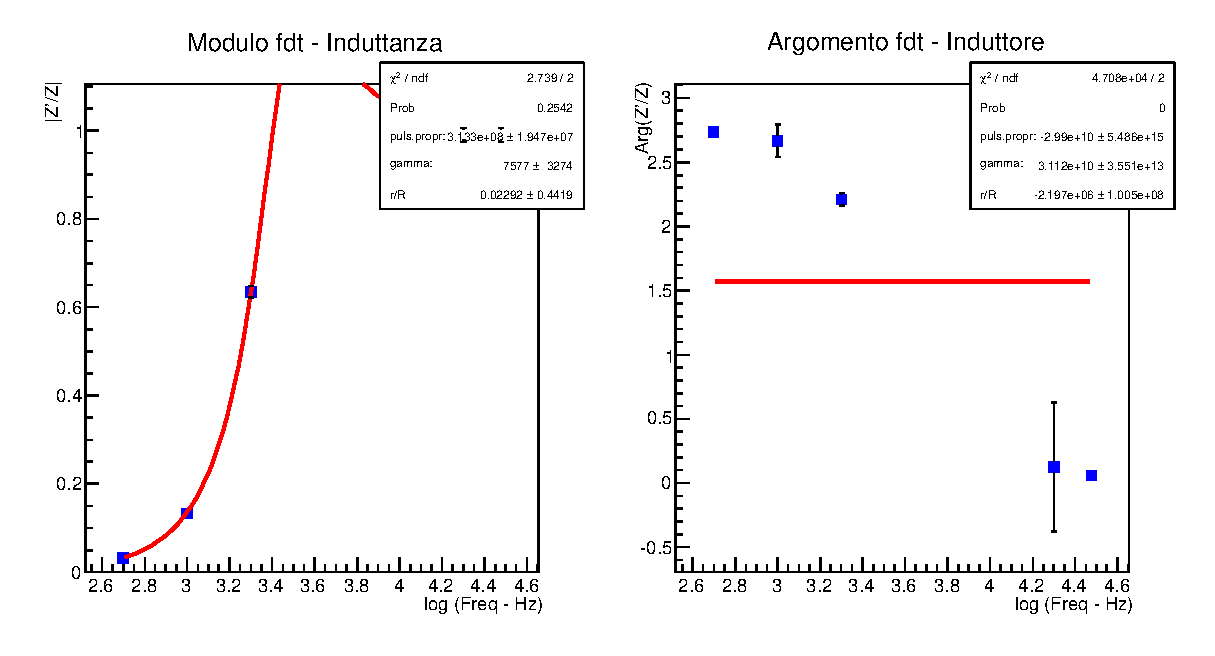
\includegraphics[scale=0.75]{Grafici/C4_P2_Ind.eps}
\caption{
Circuito RLC serie.
AC.
Funzione di traferimento ai capi dell'induttore.
}
\label{fig:C4_P2_Ind}
\end{figure}



\subsubsection{Conclusioni}

La tabella riporta le stime dei parametri del circuito.
Le tre colonne centrali riportano le stime della Parte 2 in corrente alternata. L'ultima colonna riporta le stime conclusive degli stessi parametri eseguite nella Parte 1 in corrente impulsata.

La parte 2 dell'esperimento riguardante le funzioni di trasferimento per capacità e induttore non è andata a buon fine. I risultati dei fit non vengono riportati perchè non affidabili.



\begin{table}[H]
\begin{center}
\begin{tabular}{|c|c|c|c|c|c|}

\hline
\multicolumn{ 1}{|c|}{Par.} & \multicolumn{ 1}{c|}{U.tà} & \multicolumn{ 3}{c|}{Funzioni di trasferimento RLC – AC} & \multicolumn{ 1}{c|}{RLC – DC} \\ \cline{3-5}

\multicolumn{ 1}{|c|}{} & \multicolumn{ 1}{c|}{} & Res & Cond & Ind & \multicolumn{ 1}{c|}{} \\ \hline

$r$ & $\Omega$ & $104\pm8\%$ &  &  & $100\pm1\%$ \\ 
$L$ & $H$ & $0.077\pm2\%$ &  &  & $0.066\pm2\%$ \\ 
$C$ & $nF$ & $41\pm4\%$ &  &  & $46\pm3\%$ \\ \hline
$R$ & $\Omega$ & \multicolumn{ 3}{c|}{$1000\pm1\%$} & $200\pm1\%$ \\ 
\hline

\end{tabular}
\end{center}
\caption{
Stime di $r$, $L$ e $C$.
$r$: resistenza parassita del circuito, comprensiva della resistenza del generatore e quella interna dell'induttore.
$L$: induttanza.
$C$: capacità.
$R$: resistenza del resistore non è stata oggetto di stima in quanto misurata direttamente, e riportata qui per completezza.
Nell'ultima colonna sono riportati i valori stimati nella Parte 1 in corrente continua.
}
\label{C4_P2_finale}
\end{table}

\break